%!TEX root = ../thesis.tex
%*******************************************************************************
%****************************** Third Chapter **********************************
%*******************************************************************************
\chapter{Diseño Conceptual}

% **************************** Define Graphics Path **************************
\ifpdf
    \graphicspath{{Chapter3/Figuras/}{Chapter3/Figs/PDF/}{Chapter3/Figs/}}
\else
    \graphicspath{{Chapter3/Figs/Vector/}{Chapter3/Figs/}}
\fi

\section{Requerimientos del sistema}
Uno de los requerimientos principales del sistema es el uso de una red de sensores modular y sencilla de instalar en distintos tipos de vehículos. Esto se explica fácilmente debido a que este sistema esta orientado a ser usado en el sistema de transporte público en Lima, el cual tiene una gran variedad y un gran número de vehículos. El sistema, entonces, debe ser adaptable a cualquiera de estos vehículos y no contar con un tiempo de instalación elevado.

También se tiene como requerimiento un grado de precisión alto en el reconocimiento de estilos y eventos de conducción. Esto es necesario debido a que este sistema se usará para monitorizar y mejorar la conducta de conducción de los choferes del servicio de transporte público. Los datos arrojados por este sistema necesitan ser confiables.

Por último, se necesita también de una adecuada infraestructura que permita que el sistema funcione en linea, entregando feedback al conductor, aún si se presentan condiciones como la falta temporal de conexión a Internet. Este requerimiento será importante al considerar donde realizar el procesamiento de los datos (dentro de un sistema embebido en cada vehículo o usando un servidor).

\bgroup
\def\arraystretch{1.5}%  1 is the default, change whatever you need
\begin{table}[hpbt!]
\centering
\caption{Lista de exigencias}
\resizebox{\textwidth}{!}{%
\begin{tabularx}{\textwidth}{|l|X|}
\hline
\multicolumn{2}{|c|}{\textbf{Lista de exigencias}} \\ \hline
\textbf{Tema:} & Sistema de Reconocimiento de Estilo de Conducción para Optimización de consumo de Combustible en Vehículos del Sistema de Transporte Público de Lima \\ \hline
\textbf{Categoría} & \multicolumn{1}{c|}{\textbf{Descripción}}  \\ \hline
Función Principal & Reconocer el estilo de manejo de un conductor del sistema de transporte público de Lima y otorgarle un feedback adecuado. \\ \hline
Seguridad & El sistema no deberá influir en elementos que puedan generar un accidente de tránsito, como la visibilidad a través del parabrisas o a través de los espejos. \\ \hline
Señales & El sistema contará con una conexión a Internet permanente, con la cual guardará la información recolectada. Esta información consiste en los sensores usados (IMU, GPS, etc.) \\ \hline
Energía & El sistema funcionará a través de una batería de larga duración, que tenga la posibilidad de recargarse usando como fuente de energía al vehículo. \\ \hline
Geometría & Las medidas del sistema no deberán superar los \SI{30}{cm} de altura o de largo y ancho \\ \hline
Peso & El peso del módulo debe ser menor que \SI{1}{Kg}.\\ \hline
Electrónica & Se empleará sensores que puedan detectar información relevante para el reconocimiento de estilo de manejo y un sistema de feedback para informal al conductor. \\ \hline
Software & Se desarrollará una plataforma en la que se permita obtener los datos medidos por el sistema de una forma sencilla. \\ \hline
Mantenimiento & Se deberá realizar un mantenimiento preventivo del sistema cada 6 meses, para asegurar su funcionamiento. \\ \hline
Ergonomía & El sistema de sensores deberá estar en una posición que no afecte a la actividad de conducción y el sistema de feedback debe estar en una posición en la que el conductor pueda recibir el feedback sin comprometer la visibilidad de la tarea de conducción. \\ \hline
Transporte & El sistema será sencillo de instalar y desinstalar, para su uso en un número grande de vehículos \\ \hline
Uso & El sistema deberá usarse durante toda la tarea de conducción a temperatura ambiente y protegido de condiciones climáticas adversas. \\ \hline
Tiempo de entrega & El diseño deberá ser finalizado junto a los documentos correspondientes antes de la semana 15 del presente ciclo académico. \\ \hline
\end{tabularx}%
}
\label{diag:3.1}
\end{table}
\egroup

\newpage

\section{Estructura de funciones}
Se detallará a continuación los módulos principales que tendrá el sistema de reconocimiento de estilos de conducción con su funcionamiento y las posibles soluciones para cada uno de ellos.

\subsection{Modelo Black Box}
En la Fig~\ref{fig:3.1} se puede observar el modelo de Black Box o Caja Negra del sistema.

\begin{figure}[htbp!]
\centering
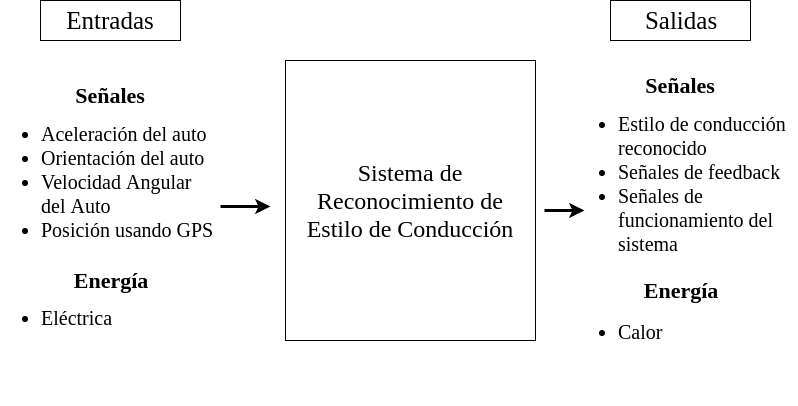
\includegraphics[width=\textwidth]{Fig1}
\caption{Modelo de Black Box del sistema}
\label{fig:3.1}
\end{figure}


El sistema estará conectado al auto, de donde obtendrá la energía necesaria para funcionar. Debido a que el enfoque del sistema es ahorrar energía. Este no debe consumir mucha.

Además de recibir la energía, este sistema recibirá las señales de los sensores que contendrán toda la información necesaria para caracterizar el estilo de conducción del usuario. Obteniendo en la salida el estilo de conducción. Este será almacenado y será representado como una señal de feedback al usuario. Además el sistema deberá indicar al usuario que esta en funcionamiento.

\subsection{Dominio Electrónico}

Este dominio se encarga principalmente de recolectar la información necesaria para lograr caracterizar el estilo de conducción de un conductor y también de brindar la energía a todos los componentes del sistema.

Se usará la energía que se encuentra disponible a través del auto en donde se encuentra instalado el sistema. Pero se tendrá en cuenta que el consumo debe ser muy pequeño para no causar un gran impacto en el consumo de combustible del auto.


\begin{figure}[htbp!]
\centering
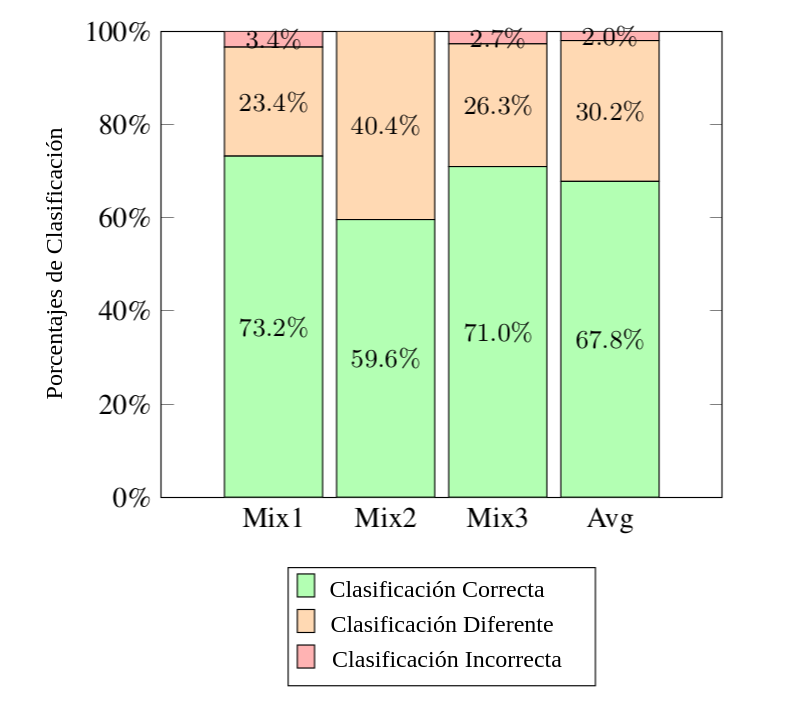
\includegraphics[width=\textwidth]{Fig2}
\caption{Diagrama de Funciones del dominio electrónico}
\label{fig:3.2}
\end{figure}
